\documentclass[12pt,a4paper]{ctexart}
\usepackage[top=2.5cm,bottom=2.5cm,left=3cm,right=2.5cm]{geometry}
\usepackage{amsmath,amssymb,graphicx,booktabs,tabularx,hyperref,float,enumitem,xcolor}
\hypersetup{colorlinks=true,linkcolor=black,citecolor=black,urlcolor=black}
\usepackage{setspace}\onehalfspacing
\graphicspath{{figures/}}
\ctexset{section/format=\Large\bfseries\centering,
         subsection/format=\large\bfseries,
         subsubsection/format=\normalsize\bfseries}
\title{\textbf{低空物联网场景下的5G-A通感一体化技术：\\标准、关键技术与应用}}
\author{倪云鹤\quad 刘知愉\quad 迟百馨\quad 刘志博文\\[6pt] 电子科技大学}
\date{2026年5月}
\begin{document}
\maketitle\thispagestyle{empty}\newpage
\setcounter{page}{1}
\tableofcontents\newpage

\begin{abstract}
通信感知一体化（ISAC）是5G-Advanced阶段最具代表性的演进技术之一。本报告聚焦低空物联网场景，围绕"低空需求$\to$感知原理$\to$标准进展$\to$IoT平台架构$\to$产业应用"这一主线，对5G-A通感一体化技术进行了系统性的研讨分析。报告推导了OFDM雷达信号模型与2D-FFT距离-速度联合估计算法，基于5G NR n79频段参数进行了仿真验证；系统梳理了3GPP R18/R19/R20中ISAC标准化进展（TR 22.837, TR 38.857）；重点设计了感知数据从物理层到应用层的端到端IoT系统架构，并对MQTT、CoAP、LwM2M等物联网协议进行了选型分析；最后对三大运营商的低空试点进行了对比分析。
\end{abstract}
\textbf{关键词：}通信感知一体化；5G-Advanced；OFDM雷达；低空物联网；系统架构

\section{绪论}

\subsection{研究背景}
低空经济作为国家战略性新兴产业正在快速崛起。据中国民航局预测，到2025年我国低空经济市场规模将达1.5万亿元，无人机注册数量已突破120万架。在物流配送、农业植保、城市巡检、应急救援等领域，无人机的规模化应用正从试点走向常态化运营。然而，低空无人机飞行高度低（通常120--600\,m）、速度慢（10--30\,m/s）、雷达反射截面积小（RCS通常小于0.01\,m$^2$），传统雷达系统难以对其进行有效监管，形成了低空安全的监管盲区。

\subsection{问题提出}
传统的低空监管依赖专用雷达站点，存在部署成本高、覆盖密度低、无法与通信网络联动等问题。以典型的X波段监视雷达为例，单套设备采购及部署费用在数百万元级别，且需要独立的站址、供电和回传链路。而现有5G蜂窝网络在城区的基站间距仅约200\,m，已实现密集覆盖。如何复用这一庞大的通信基础设施实现低空感知功能，成为产学研共同关注的焦点问题。

\subsection{ISAC技术动因}
通信感知一体化（Integrated Sensing and Communication, ISAC）技术为解决上述问题提供了全新思路。其核心思想是在现有5G基站上叠加类似雷达的感知能力：基站在发射通信信号的同时，利用目标反射的回波信号提取距离、速度和角度等感知参数。5G NR采用的OFDM波形天然具备雷达感知能力——其多载波结构支持在子载波维度估计距离、在符号维度估计速度。因此，ISAC可以在不增加额外硬件（或仅需少量改造）的前提下，将通信基站升级为"通信+感知"双功能节点，其技术动因可归纳为三点：

\begin{enumerate}[label=(\arabic*)]
  \item \textbf{覆盖复用}：城区5G基站密度极高（站间距$\sim$200\,m），天然形成密集的感知网络，无需额外建设雷达站。
  \item \textbf{硬件共享}：ISAC复用基站的天线阵列、射频前端和基带处理单元，增量硬件成本极低。
  \item \textbf{数据联动}：感知数据可通过5G核心网即时回传至云端平台，与通信数据、飞行计划数据融合处理。
\end{enumerate}

\subsection{课题目标与报告结构}
本报告沿"低空物联网需求$\to$ISAC感知原理$\to$3GPP标准化$\to$IoT平台架构$\to$产业应用"这一主线，构建完整的技术分析闭环。第二章推导OFDM雷达信号模型与关键算法并进行仿真验证；第三章梳理3GPP标准化进展；第四章设计感知数据接入IoT平台的系统架构；第五章对比分析产业应用案例；第六章讨论挑战与展望。

\section{ISAC感知原理与关键算法}

本章从OFDM雷达信号模型出发，推导距离和速度的联合估计算法，并基于5G NR n79频段的参数进行仿真验证。

\subsection{OFDM雷达信号模型}

考虑一个OFDM雷达系统，发射信号由$N$个OFDM符号组成，每个符号包含$M$个子载波。第$n$个符号的发射基带信号可表示为：
\begin{equation}
  s_n(t) = \sum_{m=0}^{M-1} d[n,m] \cdot e^{j2\pi m \Delta f (t - nT_{\mathrm{sym}})}
  \label{eq:tx}
\end{equation}
其中$d[n,m]$为第$n$个符号第$m$个子载波上的调制符号（如QPSK），$\Delta f$为子载波间隔，$T_{\mathrm{sym}}$为OFDM符号周期（含循环前缀CP）。

当信号照射到距离为$R$、径向速度为$v$的运动目标时，回波信号经历时延$\tau = 2R/c$和多普勒频移$f_d = 2v/\lambda$。接收端经下变频和去CP后，第$n$个符号第$m$个子载波上的接收信号为：
\begin{equation}
  y[n,m] = \alpha \cdot d[n,m] \cdot e^{-j2\pi m \Delta f \tau} \cdot e^{j2\pi f_d n T_{\mathrm{sym}}} + w[n,m]
  \label{eq:rx}
\end{equation}
其中$\alpha$为包含路径损耗和目标RCS的复衰减系数，$w[n,m]$为加性高斯白噪声。式\eqref{eq:rx}中，第一个指数项$e^{-j2\pi m \Delta f \tau}$包含距离信息，第二个指数项$e^{j2\pi f_d n T_{\mathrm{sym}}}$包含速度信息。

\subsection{2D-FFT距离-速度联合估计算法}

为提取感知参数，首先进行\textbf{倒频滤波}（通信符号消除）。由于发射符号$d[n,m]$已知，将接收信号逐元素除以发射符号：
\begin{equation}
  z[n,m] = \frac{y[n,m]}{d[n,m]} = \alpha \cdot e^{-j2\pi m \Delta f \tau} \cdot e^{j2\pi f_d n T_{\mathrm{sym}}} + w'[n,m]
  \label{eq:demod}
\end{equation}

倒频滤波后的矩阵$\mathbf{Z} \in \mathbb{C}^{N \times M}$可分解为两个独立的相位旋转分量。据此，可通过二维FFT实现距离和速度的联合估计：

\begin{enumerate}[label=\textbf{Step \arabic*:}]
  \item \textbf{距离估计}——沿子载波维度（$m$方向）做IFFT：
  \begin{equation}
    \hat{R} = \frac{c \cdot \hat{k}_m}{2M\Delta f}, \quad \text{距离分辨率} \quad \Delta r = \frac{c}{2B}
  \end{equation}
  其中$B = M\Delta f$为系统带宽，$\hat{k}_m$为IFFT峰值索引。
  \item \textbf{速度估计}——沿符号维度（$n$方向）做FFT：
  \begin{equation}
    \hat{v} = \frac{\lambda \cdot \hat{k}_n}{2NT_{\mathrm{sym}}}, \quad \text{速度分辨率} \quad \Delta v = \frac{\lambda}{2NT_{\mathrm{sym}}}
  \end{equation}
  \item \textbf{CFAR检测}——在二维距离-多普勒图上使用恒虚警率检测算法自适应设定阈值，提取目标参数。
\end{enumerate}

\begin{figure}[H]
  \centering
  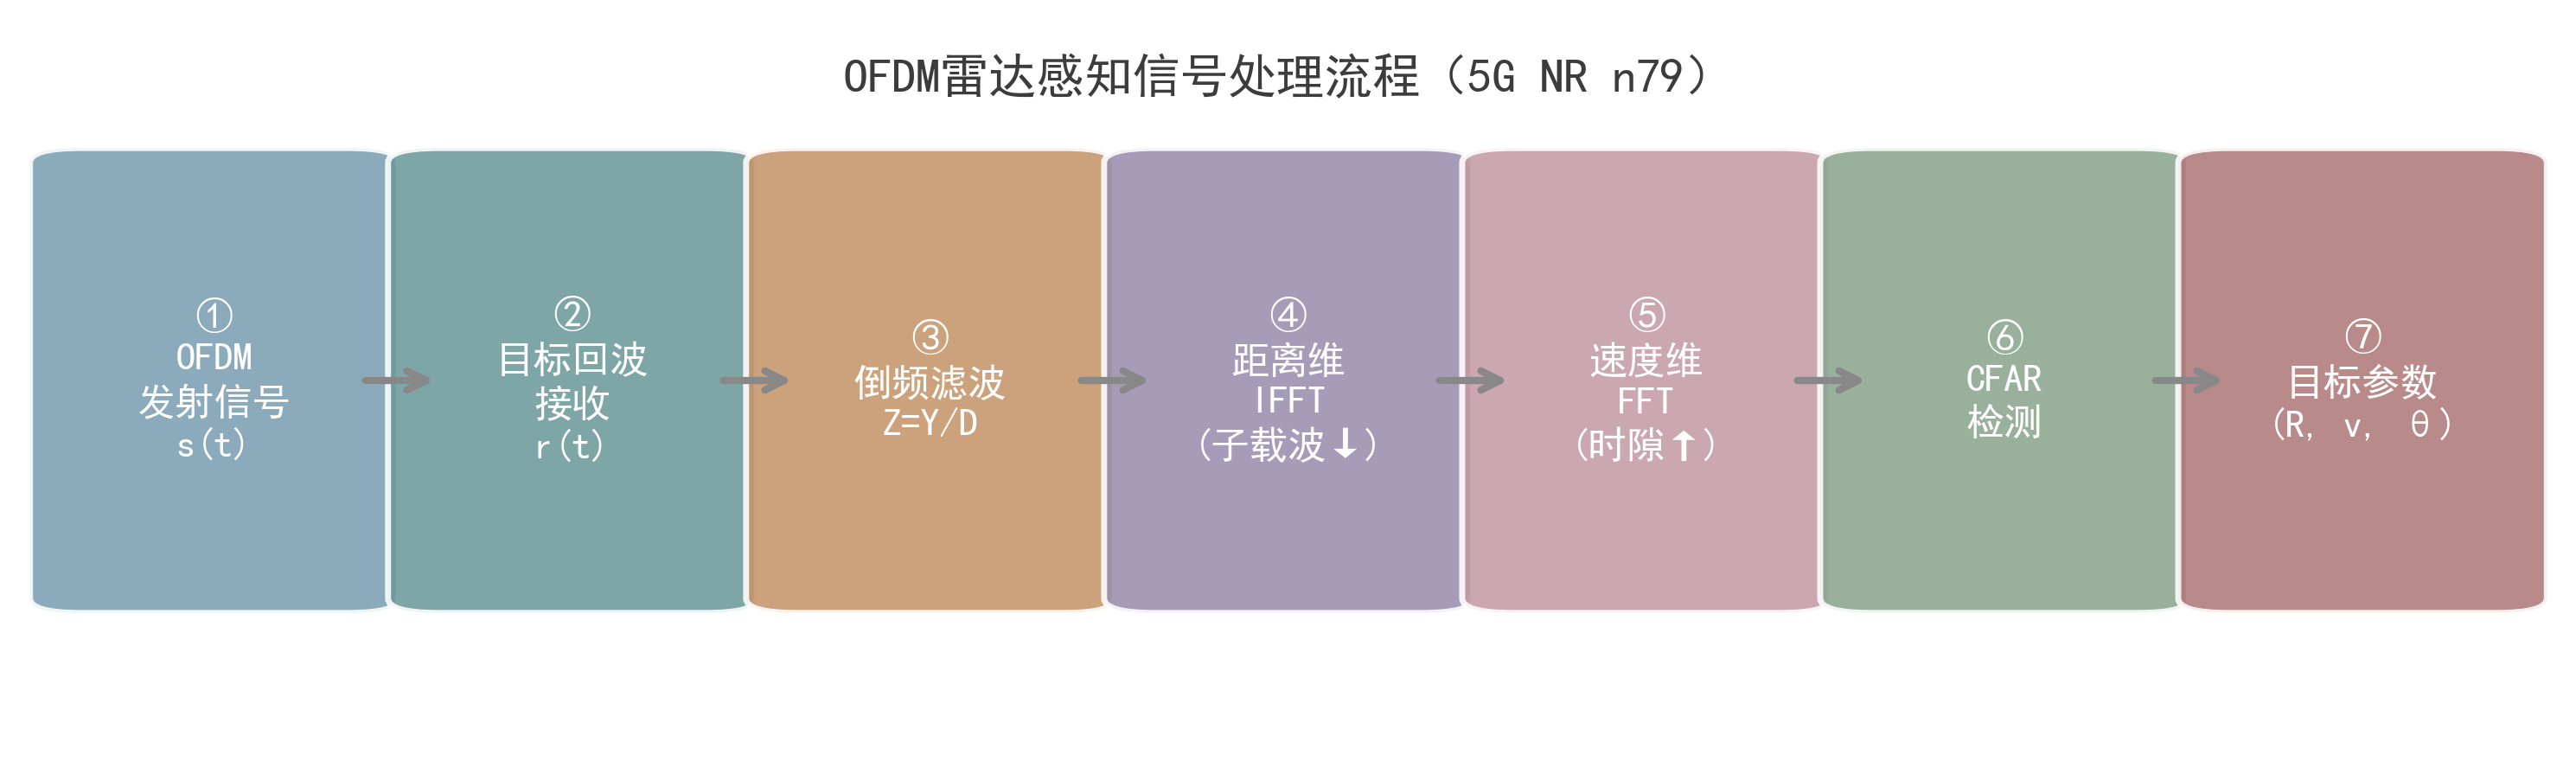
\includegraphics[width=0.95\textwidth]{signal_processing_flow.png}
  \caption{OFDM雷达感知信号处理流程}
  \label{fig:flow}
\end{figure}

\subsection{仿真参数与结果}

基于5G NR n79频段（4.9\,GHz）的标准参数进行仿真验证，具体参数如表\ref{tab:param}所示。

\begin{table}[H]
\centering\caption{OFDM雷达仿真参数（5G NR n79）}\label{tab:param}
\begin{tabular}{cccc}
\toprule
参数 & 符号 & 数值 & 说明 \\
\midrule
载波频率 & $f_c$ & 4.9\,GHz & n79频段 \\
子载波间隔 & $\Delta f$ & 30\,kHz & NR标准SCS \\
系统带宽 & $B$ & 100\,MHz & 3276个子载波 \\
OFDM符号数 & $N$ & 14 & 1个时隙(0.5\,ms) \\
距离分辨率 & $\Delta r$ & 1.50\,m & $c/(2B)$ \\
最大探测距离 & $R_{\max}$ & 5000\,m & $c/(2\Delta f)$ \\
速度分辨率(单时隙) & $\Delta v$ & 4.4\,m/s & 多时隙累积 \\
最大不模糊速度 & $v_{\max}$ & 30.6\,m/s & $\lambda/(4T_{\mathrm{sym}})$ \\
\bottomrule
\end{tabular}
\end{table}

仿真设置了4个典型低空目标：配送无人机（800\,m, 12\,m/s）、巡检无人机（1500\,m, $-$8\,m/s）、黑飞无人机（2200\,m, 18\,m/s）和eVTOL飞行器（3500\,m, $-$25\,m/s）。图\ref{fig:rdm}展示了2D-FFT处理后的距离-多普勒图，4个目标均被正确检测并定位。

\begin{figure}[H]
  \centering
  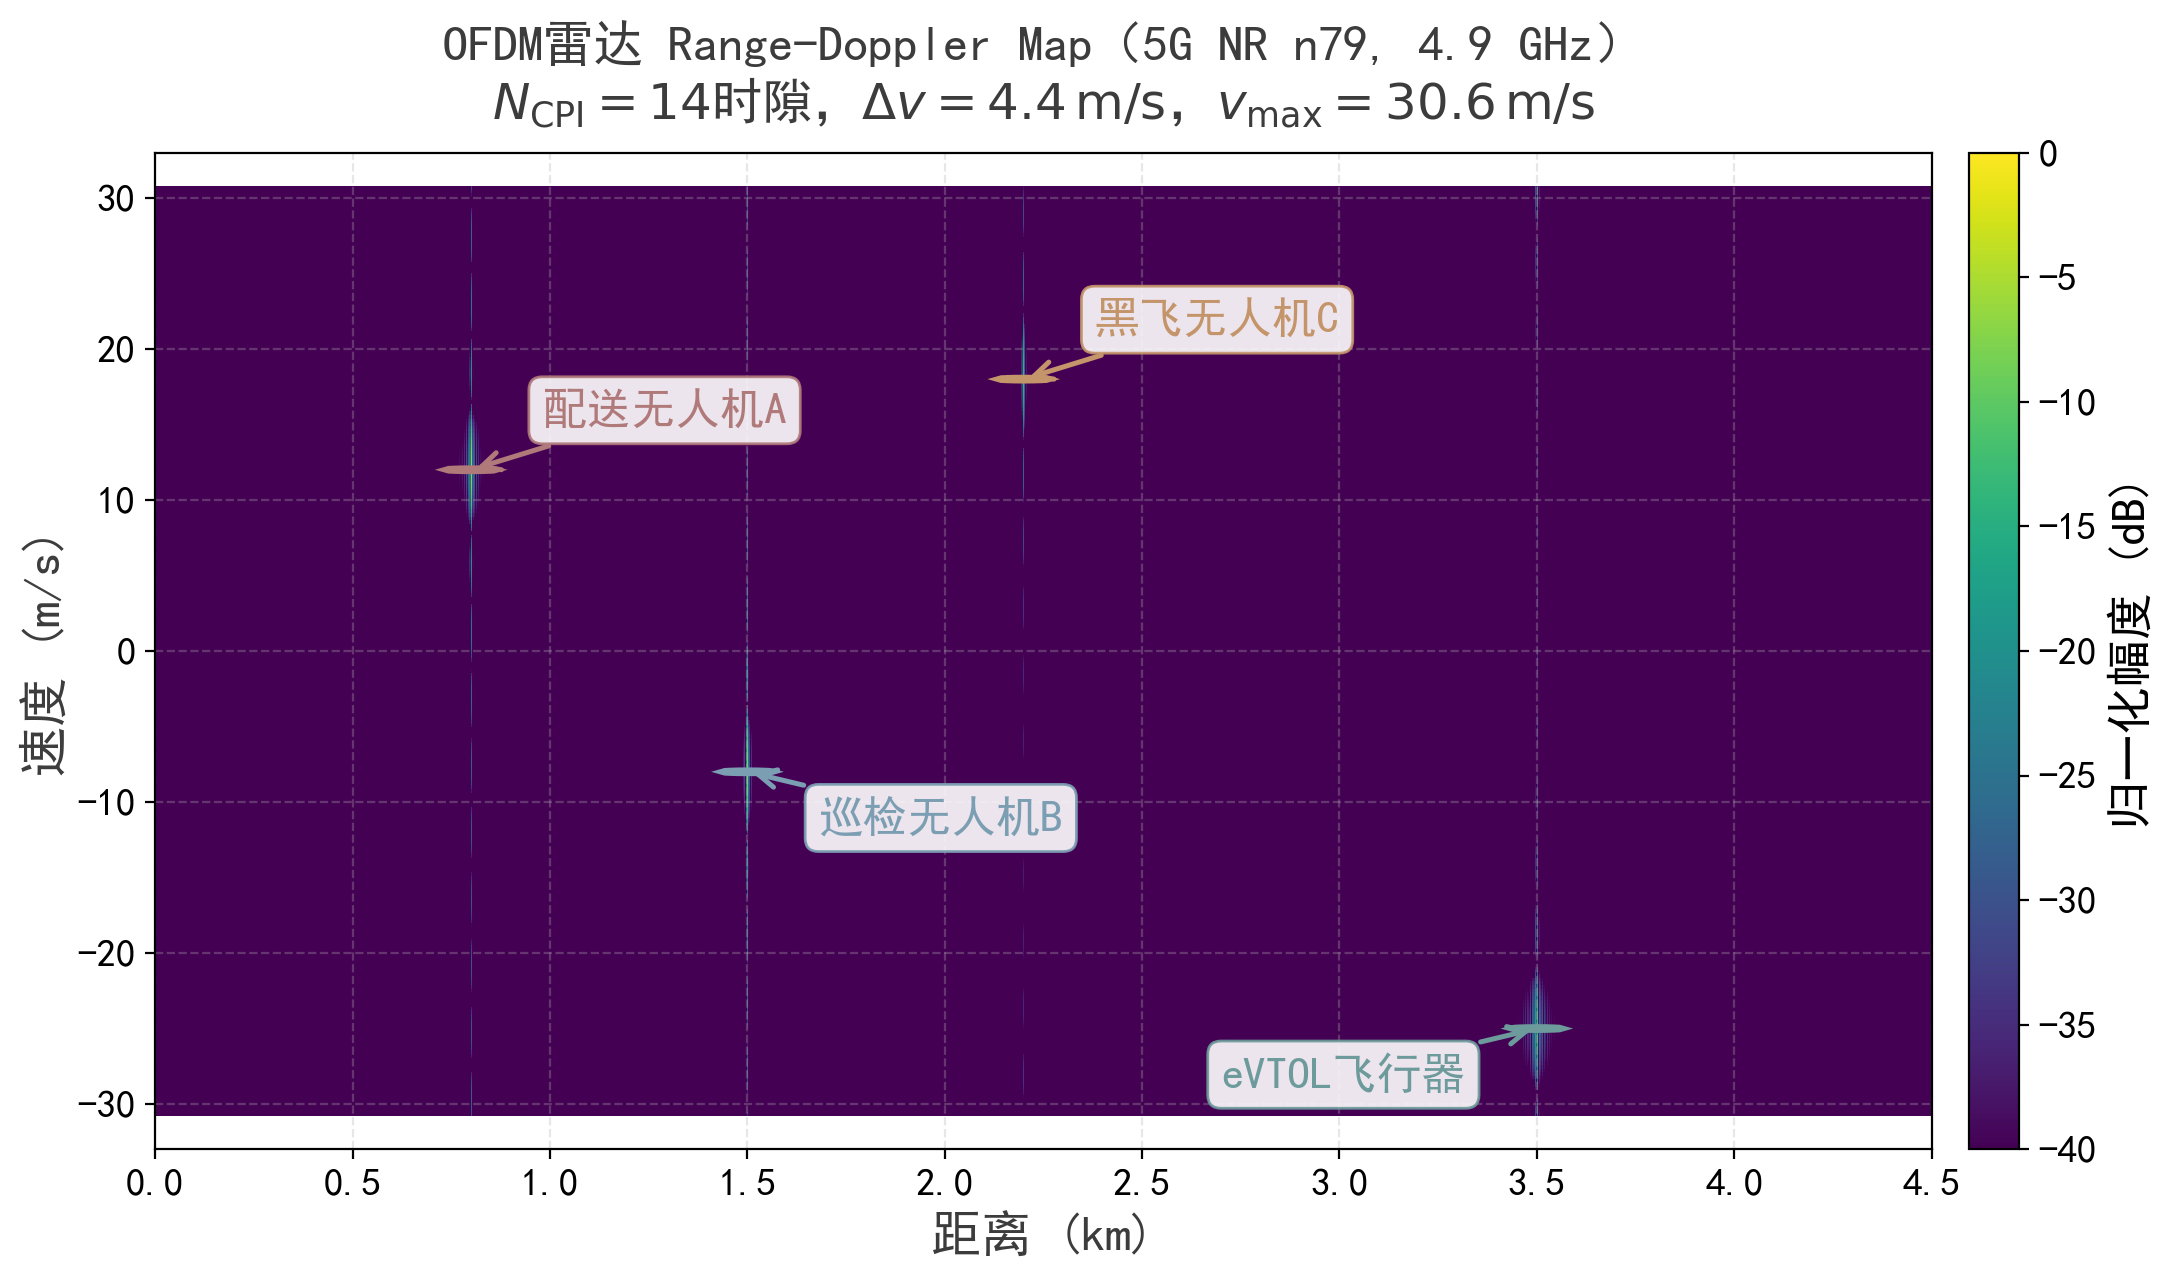
\includegraphics[width=0.85\textwidth]{range_doppler_map.png}
  \caption{OFDM雷达Range-Doppler Map仿真结果（5G NR n79, 4.9\,GHz）}
  \label{fig:rdm}
\end{figure}

\subsection{性能边界与局限性分析}

上述仿真中需要注意两个性能边界问题：

\textbf{（1）速度分辨率与多普勒混叠。}单时隙（$N=14$符号，0.5\,ms）下速度分辨率为$\Delta v \approx 4.4$\,m/s，对于低速多旋翼无人机（悬停速度$<$2\,m/s）的区分能力不足。同时，最大不模糊速度$v_{\max}=30.6$\,m/s，仿真中eVTOL的速度$-25$\,m/s已接近此边界，若目标速度超过$v_{\max}$将发生多普勒混叠。实际系统中，通过\textbf{多时隙相参积累}（如累积8个时隙，$N_{\mathrm{total}}=112$）可将速度分辨率提升至$\Delta v \approx 0.55$\,m/s，同时结合\textbf{交错PRF}技术可扩展不模糊速度范围。

\textbf{（2）距离-速度耦合。}OFDM波形的模糊函数在距离-多普勒平面上呈二维sinc形状，通信符号的随机性导致旁瓣电平较高（约$-13$\,dB），在强目标附近可能遮蔽弱目标。可通过发射符号的序列优化（如Zadoff-Chu序列）或加窗处理降低旁瓣。

\subsection{自干扰消除技术}

ISAC系统面临的关键工程挑战是自干扰问题。基站发射功率（约46\,dBm）与回波功率（可低至$-100$\,dBm以下）之间存在超过140\,dB的动态范围差异。自干扰消除采用三级级联架构：

\begin{figure}[H]
  \centering
  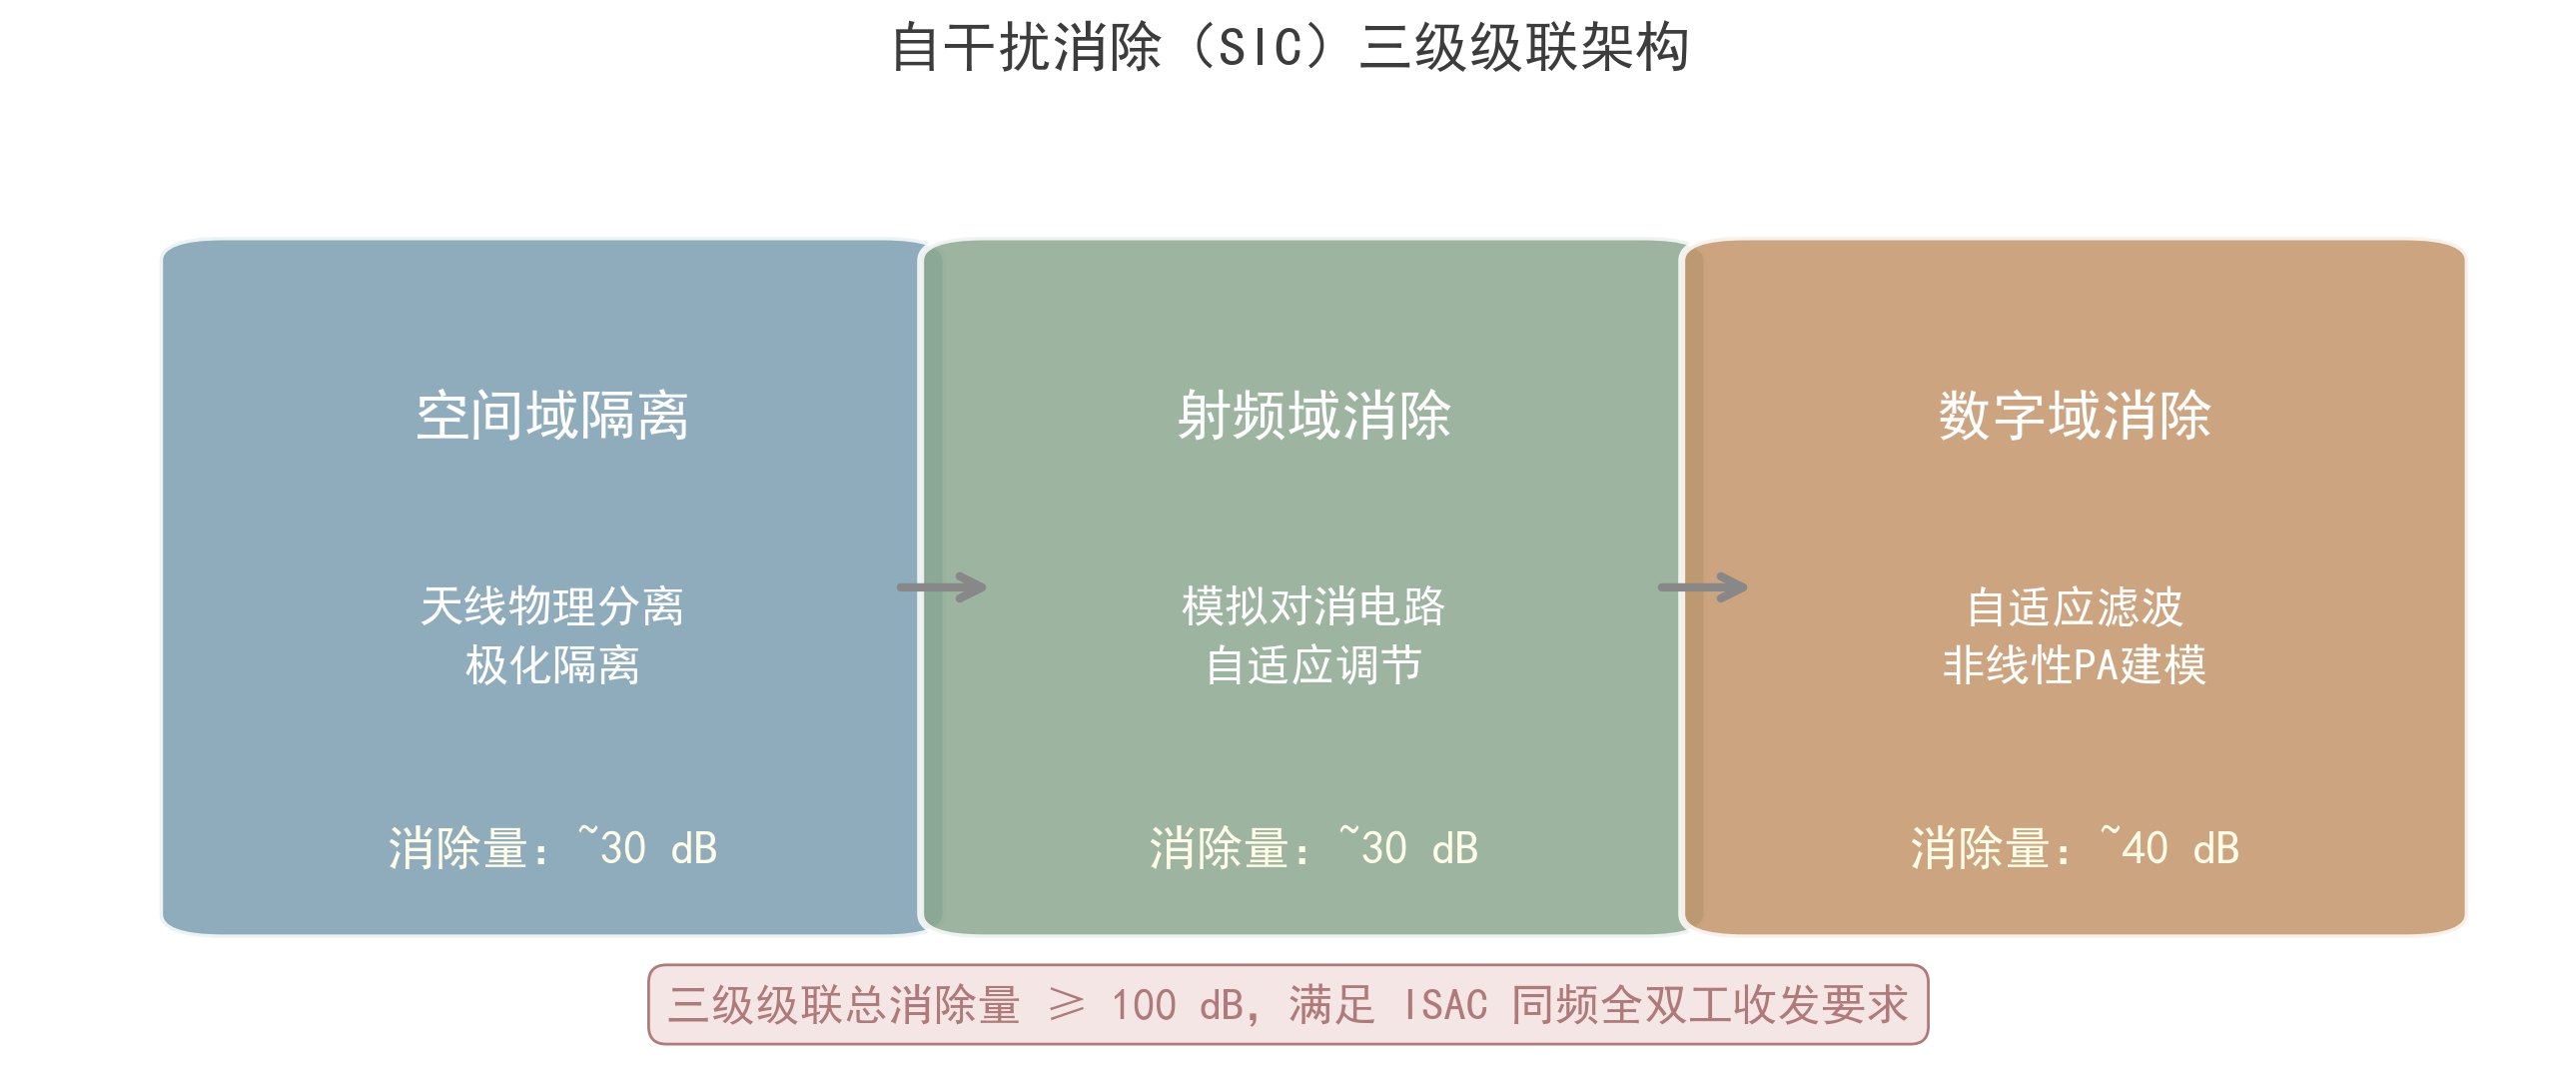
\includegraphics[width=0.85\textwidth]{sic_architecture.png}
  \caption{自干扰消除（SIC）三级架构}
  \label{fig:sic}
\end{figure}

空间域隔离通过天线物理分离和极化隔离实现约30\,dB抑制；射频域消除利用模拟对消电路实现约30\,dB抑制；数字域消除通过自适应滤波和非线性建模实现约40\,dB抑制。三级总消除量需$\geq$100\,dB。其中数字域消除最具挑战性，因为功率放大器（PA）的非线性效应和I/Q不平衡会产生难以建模的残余干扰分量。

\subsection{本章小结}
本章建立了OFDM雷达信号模型，推导了基于2D-FFT的距离-速度联合估计算法，通过仿真验证了5G NR参数下的感知性能满足低空无人机探测需求，同时分析了速度分辨率局限性和自干扰消除这两个关键技术挑战。

\section{3GPP标准化进展}

ISAC的标准化工作由3GPP主导推进，贯穿5G-A到6G的多个Release版本。本章系统梳理其演进路线，重点关注与低空感知相关的标准项目。

\subsection{R18：感知场景需求预研}

3GPP R18作为5G-Advanced的首个版本（2024年6月功能冻结），启动了感知场景与需求的Study Item（SI）。核心标准文档为\textbf{TR 22.837}~\cite{tr22837}《Feasibility Study on Integrated Sensing and Communication》，该文档定义了6大典型感知用例：

\begin{enumerate}[label=(\arabic*)]
  \item \textbf{入侵检测与监控}——室内外非授权目标探测
  \item \textbf{无人机跟踪与监管}——低空飞行器实时定位（\textbf{最高优先级}）
  \item \textbf{天气监测}——利用回波信号估计降雨率
  \item \textbf{道路使用者定位}——V2X场景中的行人/车辆感知
  \item \textbf{睡眠监测}——室内毫米波呼吸/心跳检测
  \item \textbf{手势识别}——近场人机交互
\end{enumerate}

其中，无人机跟踪与低空入侵检测被确定为最高优先级场景。TR 22.837中定义的典型KPI要求包括：定位精度$<$10\,m、速度估计精度$<$1\,m/s、探测距离$>$1\,km、刷新率$>$1\,Hz。该SI由华为担任Rapporteur，高通、爱立信、中兴等主要设备商参与。

\subsection{R19：ISAC信道建模研究}

R19（预计2025年功能冻结）将ISAC信道建模列为重点Work Item。核心标准文档为\textbf{TR 38.857}~\cite{tr38857}《Study on NR-based Sensing》。感知信道与传统通信信道存在本质差异：通信信道建模关注多径传播的统计特性（如时延扩展、角度扩展），而感知信道需要精确描述目标的确定性散射特性。

TR 38.857定义了6种感知操作模式：
\begin{itemize}
  \item \textbf{Mono-static sensing}（单站感知）：同一基站发射和接收，最简单但受自干扰限制
  \item \textbf{Bi-static sensing}（双站感知）：不同基站分别发射和接收，避免自干扰但需严格同步
  \item \textbf{Multi-static sensing}（多站感知）：多个基站协同，提供空间分集增益
  \item \textbf{UE-assisted sensing}：终端辅助的感知模式
  \item \textbf{UE-based sensing}：终端独立完成感知处理
  \item \textbf{Network-assisted sensing}：网络侧提供感知辅助信息
\end{itemize}

R19的研究重点还包括：感知参考信号（SRS-like sensing RS）设计方案、目标RCS角度依赖性建模（Swerling I--IV模型的扩展）、以及感知与通信在资源分配层面的协调机制。

\subsection{R20及6G演进路线}

R20阶段（2026年启动）已将集成感知确定为5G-A继续演进的核心方向之一，计划制定ISAC的功能规范（Normative Work）和空口协议。具体包括：感知会话管理流程、感知能力协商机制、感知结果上报接口规范等。

在更长远的6G愿景中，国际电信联盟（ITU）已在IMT-2030框架中将通信感知一体化确认为6G的\textbf{三大新增核心能力}之一（另外两个为AI原生和数字孪生）。6G的目标是实现\textbf{原生感知}——在系统设计之初就将感知作为基本能力纳入，而非5G-A阶段的"叠加式"方案。

\begin{figure}[H]
  \centering
  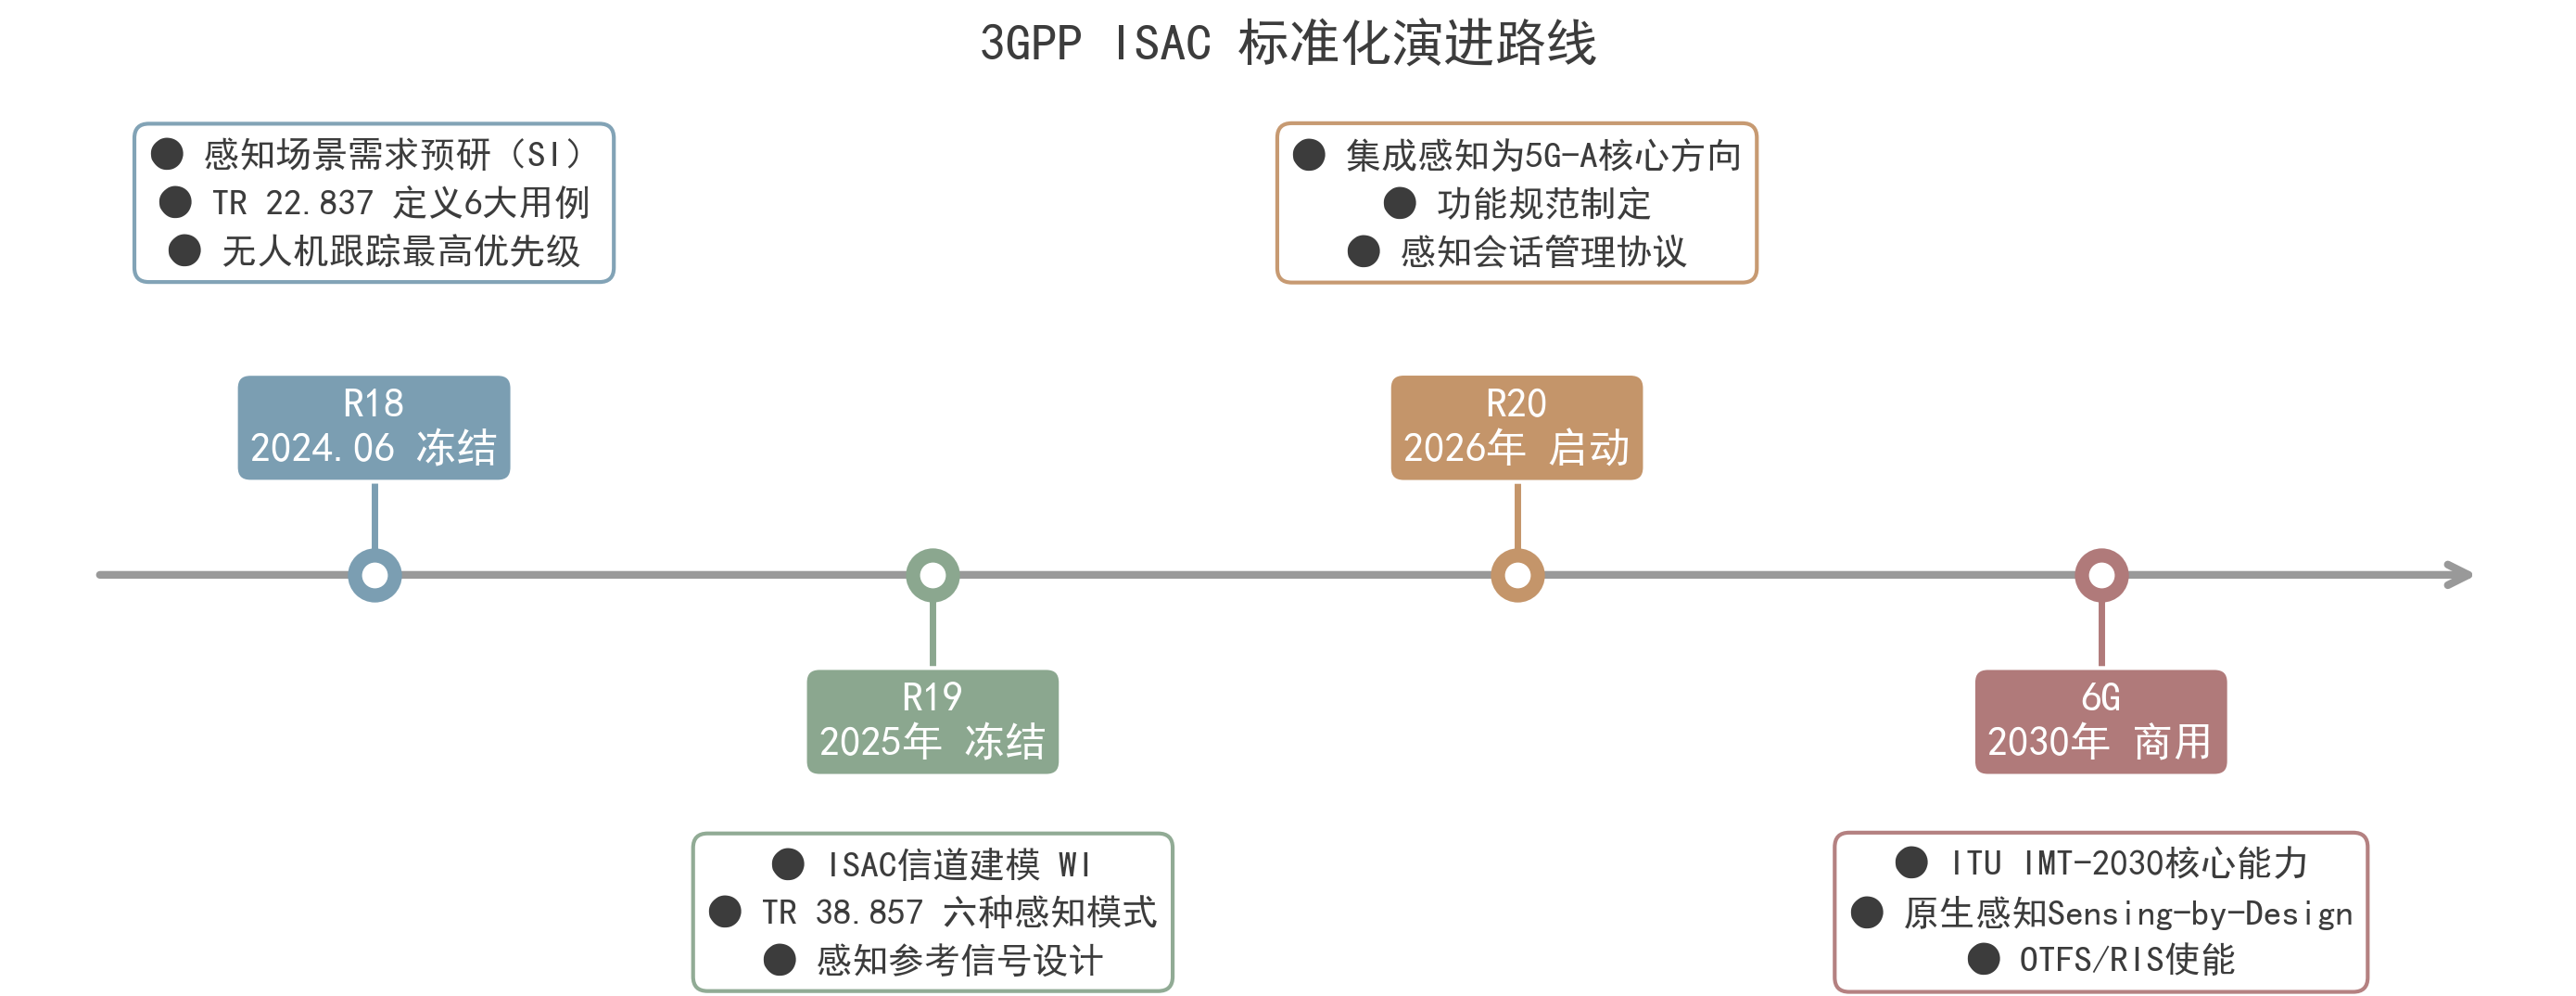
\includegraphics[width=0.95\textwidth]{3gpp_timeline.png}
  \caption{3GPP ISAC标准化演进路线}
  \label{fig:timeline}
\end{figure}

\subsection{本章小结}
3GPP的ISAC标准化遵循"场景定义（R18 TR 22.837）$\to$信道建模（R19 TR 38.857）$\to$功能规范（R20）$\to$原生感知（6G）"的演进路径。当前处于信道建模和功能预研的关键阶段，预计在6G时代（2030年前后）实现原生通感融合。

\section{感知数据接入IoT平台的系统架构}

本章是报告最体现物联网系统视角的核心章节。ISAC的感知数据不应停留在物理层，而应上升至平台层和应用层驱动低空业务逻辑。

\subsection{端到端系统架构设计}

低空物联网通感一体化系统采用五层架构（图\ref{fig:arch}），自下而上分别为目标层、感知层、网络层、平台层和应用层。

\begin{figure}[H]
  \centering
  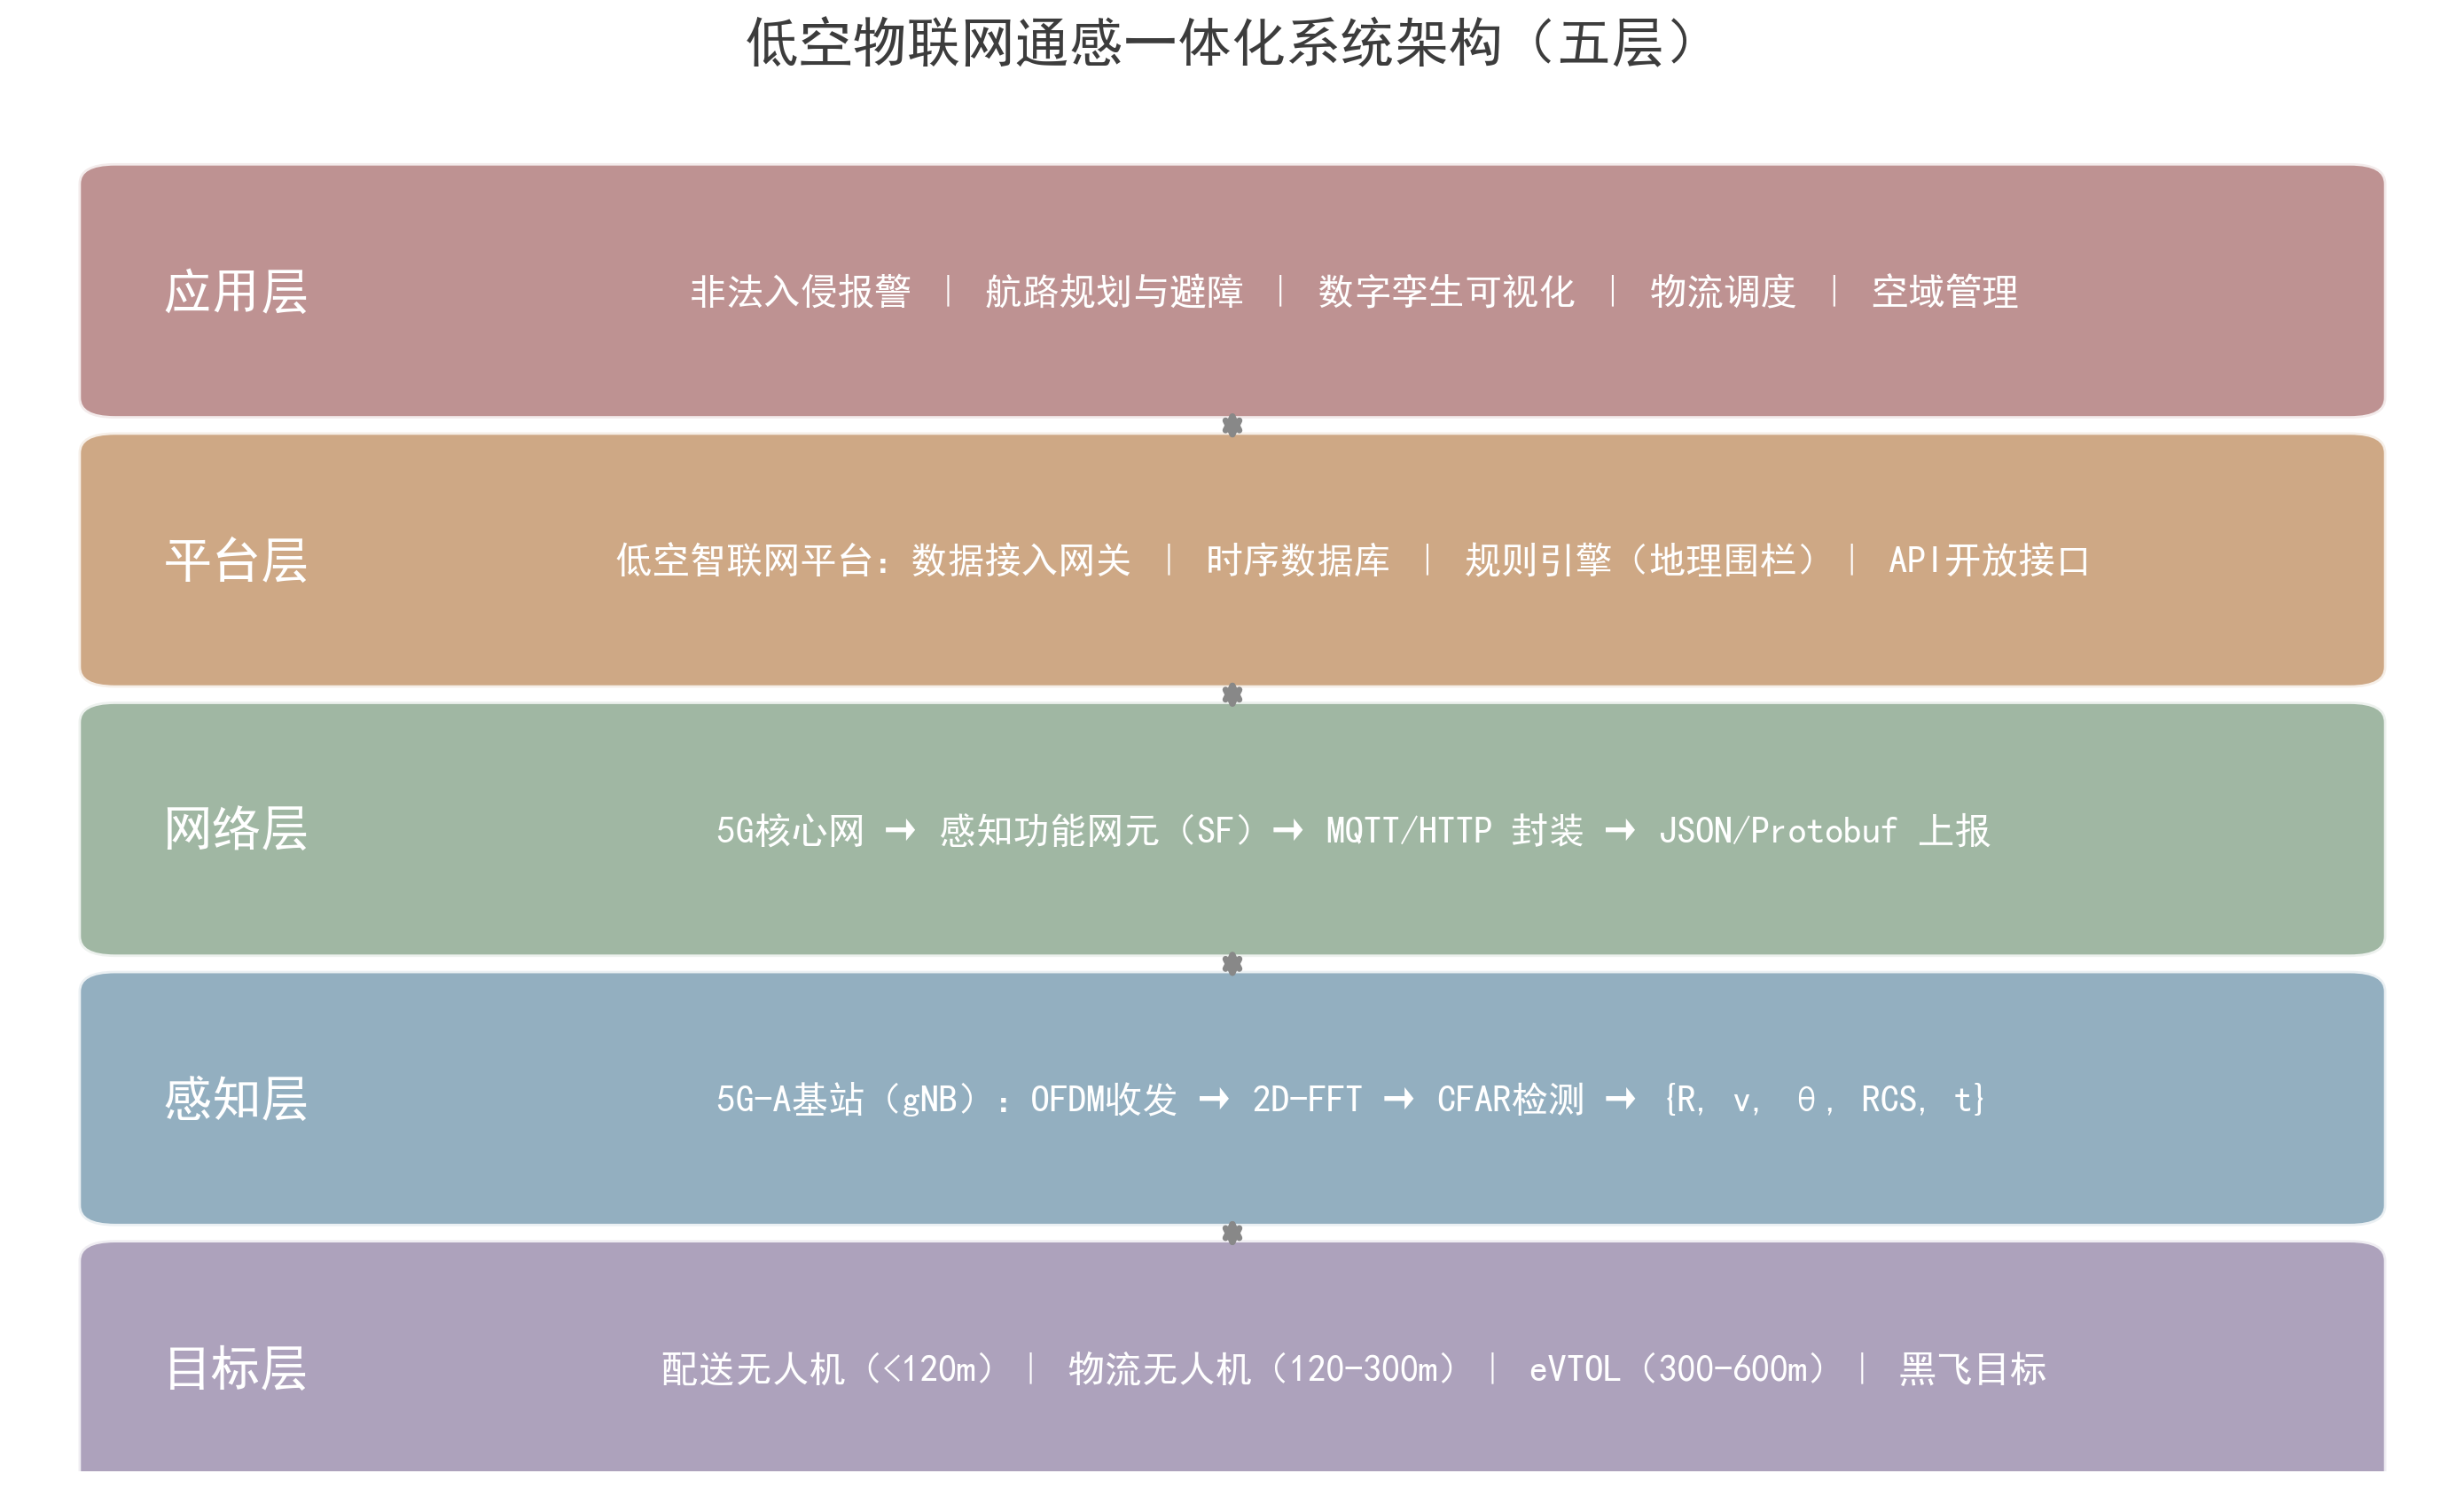
\includegraphics[width=0.95\textwidth]{iot_architecture.png}
  \caption{低空物联网通感一体化系统五层架构}
  \label{fig:arch}
\end{figure}

\begin{itemize}
  \item \textbf{目标层}：包括合作目标（已注册配送/物流无人机、eVTOL）和非合作目标（黑飞无人机），不同类型目标具有不同的RCS特征（$-20\sim-5$\,dBsm）和运动模式。
  \item \textbf{感知层}：5G-A基站配备感知处理单元，执行OFDM信号收发、2D-FFT和CFAR检测，输出目标参数集$\{$位置, 速度, 航向, RCS, 时间戳$\}$。
  \item \textbf{网络层}：5G核心网中新增感知功能网元（Sensing Function, SF），管理感知会话并将数据通过标准接口上报。
  \item \textbf{平台层}：低空智联网平台，包含数据接入网关、时序数据库（如InfluxDB/TDengine）、规则引擎（地理围栏/禁飞区判定）和API开放接口。
  \item \textbf{应用层}：面向终端用户的业务应用——非法入侵报警、航路规划与避障、数字孪生可视化、物流调度优化。
\end{itemize}

\subsection{感知数据模型与上报流程}

感知数据的标准化是实现跨平台互通的基础。本文设计的感知数据字段结构如下（以JSON格式封装）：

\begin{verbatim}
{
  "target_id": "UAV-0037",
  "timestamp": "2025-05-10T08:30:00Z",
  "position": {"lat": 22.5431, "lon": 114.0579, "alt": 85.2},
  "velocity": {"vx": 5.2, "vy": -3.1, "vz": 0.3},
  "rcs_dbsm": -15.2,
  "confidence": 0.92,
  "cell_id": "460-00-12345-67"
}
\end{verbatim}

上报频率根据场景需求差异化设计：高精度配送场景（$<$120\,m）采用1\,Hz；入侵检测场景需要更高实时性，采用10\,Hz；城际飞行场景（300--600\,m）采用0.5\,Hz。

\subsection{物联网通信协议选型分析}

感知数据的上报协议直接影响系统的实时性、可靠性和可扩展性。针对低空物联网场景，本文对四种主流物联网协议进行对比分析，如表\ref{tab:protocol}所示。

\begin{table}[H]
\centering\caption{物联网通信协议对比分析}\label{tab:protocol}
\begin{tabular}{lcccc}
\toprule
特性 & \textbf{MQTT} & \textbf{CoAP} & \textbf{LwM2M} & \textbf{HTTP/REST} \\
\midrule
传输层 & TCP & UDP & UDP(CoAP) & TCP \\
通信模式 & 发布/订阅 & 请求/响应 & 请求/响应+观察 & 请求/响应 \\
消息开销 & 小(2B头) & 极小(4B头) & 小 & 大 \\
QoS支持 & 3级 & CON/NON & 继承CoAP & 无原生 \\
设备管理 & 无 & 无 & \textbf{内置} & 无 \\
安全性 & TLS & DTLS & DTLS & TLS \\
适用场景 & 数据汇聚 & 受限设备 & 设备全生命周期 & 管理/查询 \\
\bottomrule
\end{tabular}
\end{table}

综合分析，推荐以下协议组合方案：
\begin{itemize}
  \item \textbf{感知数据上报}：采用\textbf{MQTT}协议。其发布/订阅模式天然适合"多基站→平台"的多对一数据汇聚，QoS分级机制可根据场景灵活选择可靠性级别（入侵告警用QoS 2确保不丢失，常规轨迹用QoS 0降低延迟）。
  \item \textbf{基站感知能力管理}：采用\textbf{LwM2M}协议。其内置的设备注册、固件升级、资源观察等设备管理功能，可用于远程配置基站的感知参数（如CFAR阈值、上报频率）。
  \item \textbf{应用层API}：采用\textbf{HTTP/RESTful}接口，供第三方开发者查询轨迹数据和订阅告警事件。
\end{itemize}

此外，在与现有低空飞行管理体系对接方面，需考虑与UTM（Unmanned Traffic Management）/ U-Space系统的北向接口兼容。UTM系统通常采用RESTful API和WebSocket进行飞行计划提交与实时态势共享，ISAC感知平台的输出应按照UTM标准数据格式封装，实现与空域管理系统的无缝对接。

\subsection{多站协同感知与数据融合}

单站感知存在遮挡盲区和角度模糊等局限性。多基站协同感知分为两个层级：

\textbf{检测级融合}：各基站独立完成目标检测后，将检测结果上报至融合中心。融合中心通过航迹关联算法（如最近邻法/JPA全局最优关联法）将不同基站对同一目标的检测结果进行关联匹配。

\textbf{轨迹级融合}：对关联后的多源观测数据，使用扩展卡尔曼滤波（EKF）进行状态估计。目标状态向量$\mathbf{x}_k = [x, y, z, \dot{x}, \dot{y}, \dot{z}]^T$，状态转移方程为：
\begin{equation}
  \mathbf{x}_{k+1} = \mathbf{F}\mathbf{x}_k + \mathbf{w}_k, \quad \mathbf{z}_k = \mathbf{H}\mathbf{x}_k + \mathbf{v}_k
\end{equation}
其中$\mathbf{F}$为匀速运动模型的状态转移矩阵，$\mathbf{H}$为观测矩阵。实测数据表明，三站协同可将定位精度从单站的10\,m量级提升至3\,m以内。

\subsection{本章小结}
本章设计了低空物联网通感一体化的五层系统架构，定义了感知数据模型，对MQTT/CoAP/LwM2M等物联网协议进行了选型分析，并讨论了多站协同感知的数据融合方案，实现了从物理层感知到应用层服务的完整闭环。

\section{低空应用案例与部署分析}

\subsection{三大运营商低空试点对比}

截至2025年，国内三大运营商均已布局低空通感一体方案，进展情况如表\ref{tab:operator}所示。

\begin{table}[H]
\centering\caption{三大运营商低空通感一体试点对比}\label{tab:operator}
\begin{tabular}{lccc}
\toprule
维度 & 中国移动 & 中国电信 & 中国联通/中兴 \\
\midrule
合作伙伴 & 美团 & 华为 & 中兴通讯 \\
典型场景 & 低空外卖配送 & 医疗物资配送 & 黑飞无人机监测 \\
部署城市 & 深圳 & 武汉、上海 & 全国25省 \\
试点规模 & 30+航线, 30万+订单 & 多城试点 & 80+试点项目 \\
感知频段 & 4.9\,GHz (n79) & 4.9\,GHz & 4.9\,GHz \\
感知距离 & $\sim$1.5\,km & $\sim$1.2\,km & $\sim$2\,km \\
获奖 & — & 2025 GSMA大奖 & 规模最大 \\
\bottomrule
\end{tabular}
\end{table}

\begin{figure}[H]
  \centering
  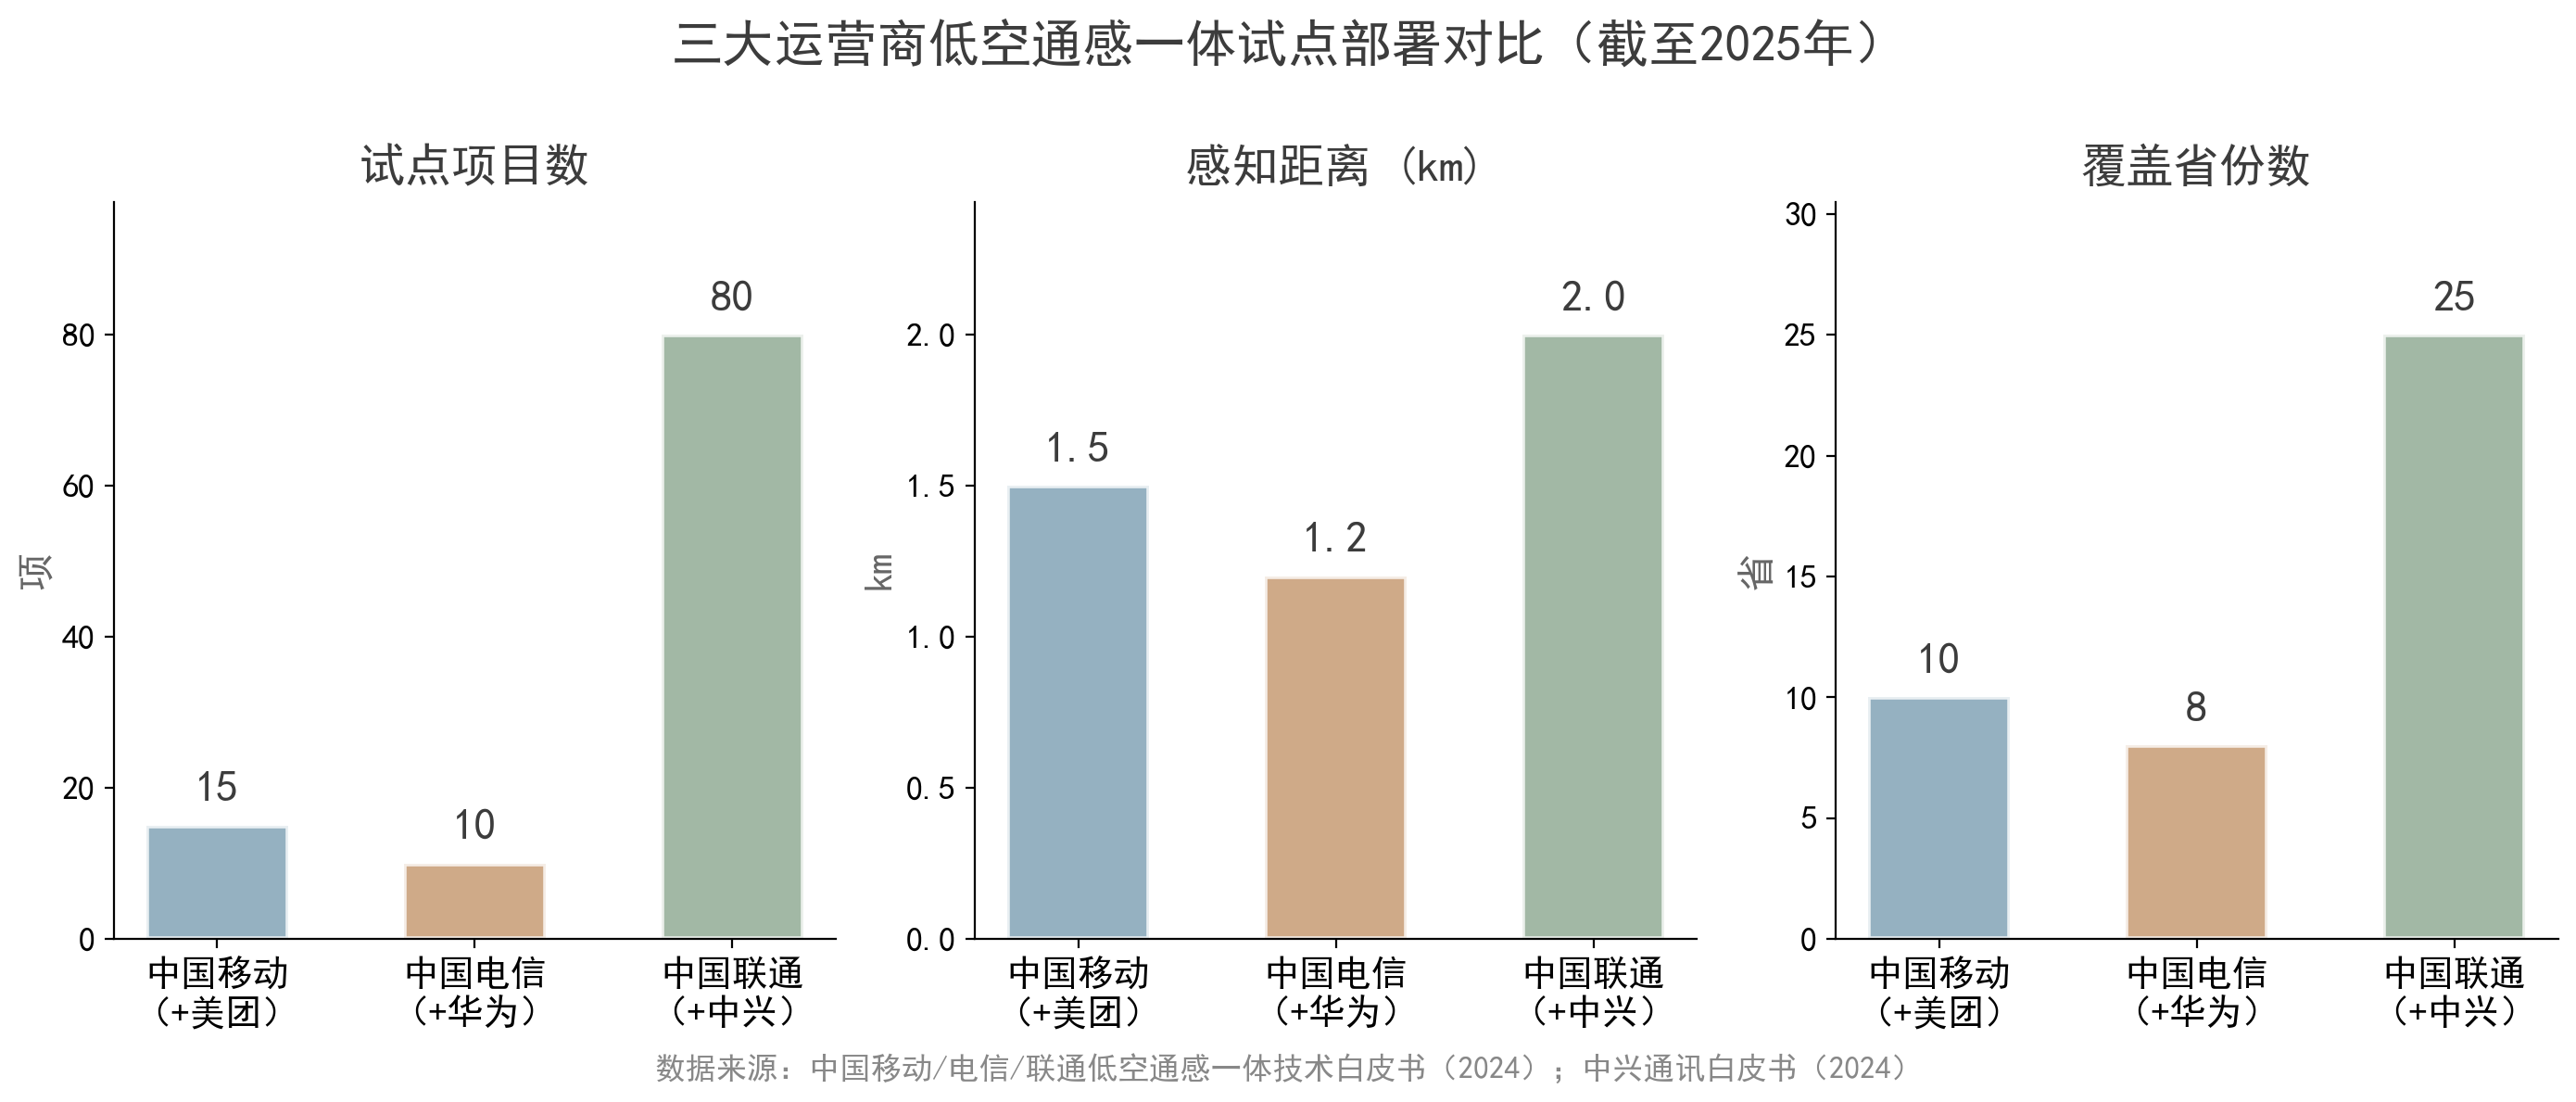
\includegraphics[width=0.85\textwidth]{operator_comparison.png}
  \caption{三大运营商低空试点部署对比}
  \label{fig:operator}
\end{figure}

中国移动与美团合作的深圳低空外卖配送项目最具产业示范意义：已开通30余条航线、累计完成超30万单配送订单，实现了从技术验证到规模化商业运营的跨越。中国电信联合华为的5G无人机医疗配送方案荣获2025年GSMA全球移动大奖。中兴通讯在覆盖广度上领先，已在25个省市完成超80个试点项目。

\subsection{ISAC与传统雷达方案对比}

从六个维度对ISAC方案与传统专用雷达进行综合对比，如表\ref{tab:vs}和图\ref{fig:radar}所示。

\begin{table}[H]
\centering\caption{ISAC与传统雷达方案综合对比}\label{tab:vs}
\begin{tabular}{lcc}
\toprule
维度 & 5G-A ISAC方案 & 专用雷达方案 \\
\midrule
部署成本 & 低（复用基站，增量$<$10\%） & 高（单套数百万元） \\
覆盖密度 & 高（城区站间距$\sim$200\,m） & 低（雷达站稀疏） \\
距离分辨率 & $\sim$1.5\,m (100\,MHz) & $\sim$0.15\,m (1\,GHz) \\
低慢小检测 & 适中 & 较好 \\
通信能力 & 原生支持 & 无 \\
组网能力 & 强（天然联网） & 弱（需额外回传） \\
\bottomrule
\end{tabular}
\end{table}

\begin{figure}[H]
  \centering
  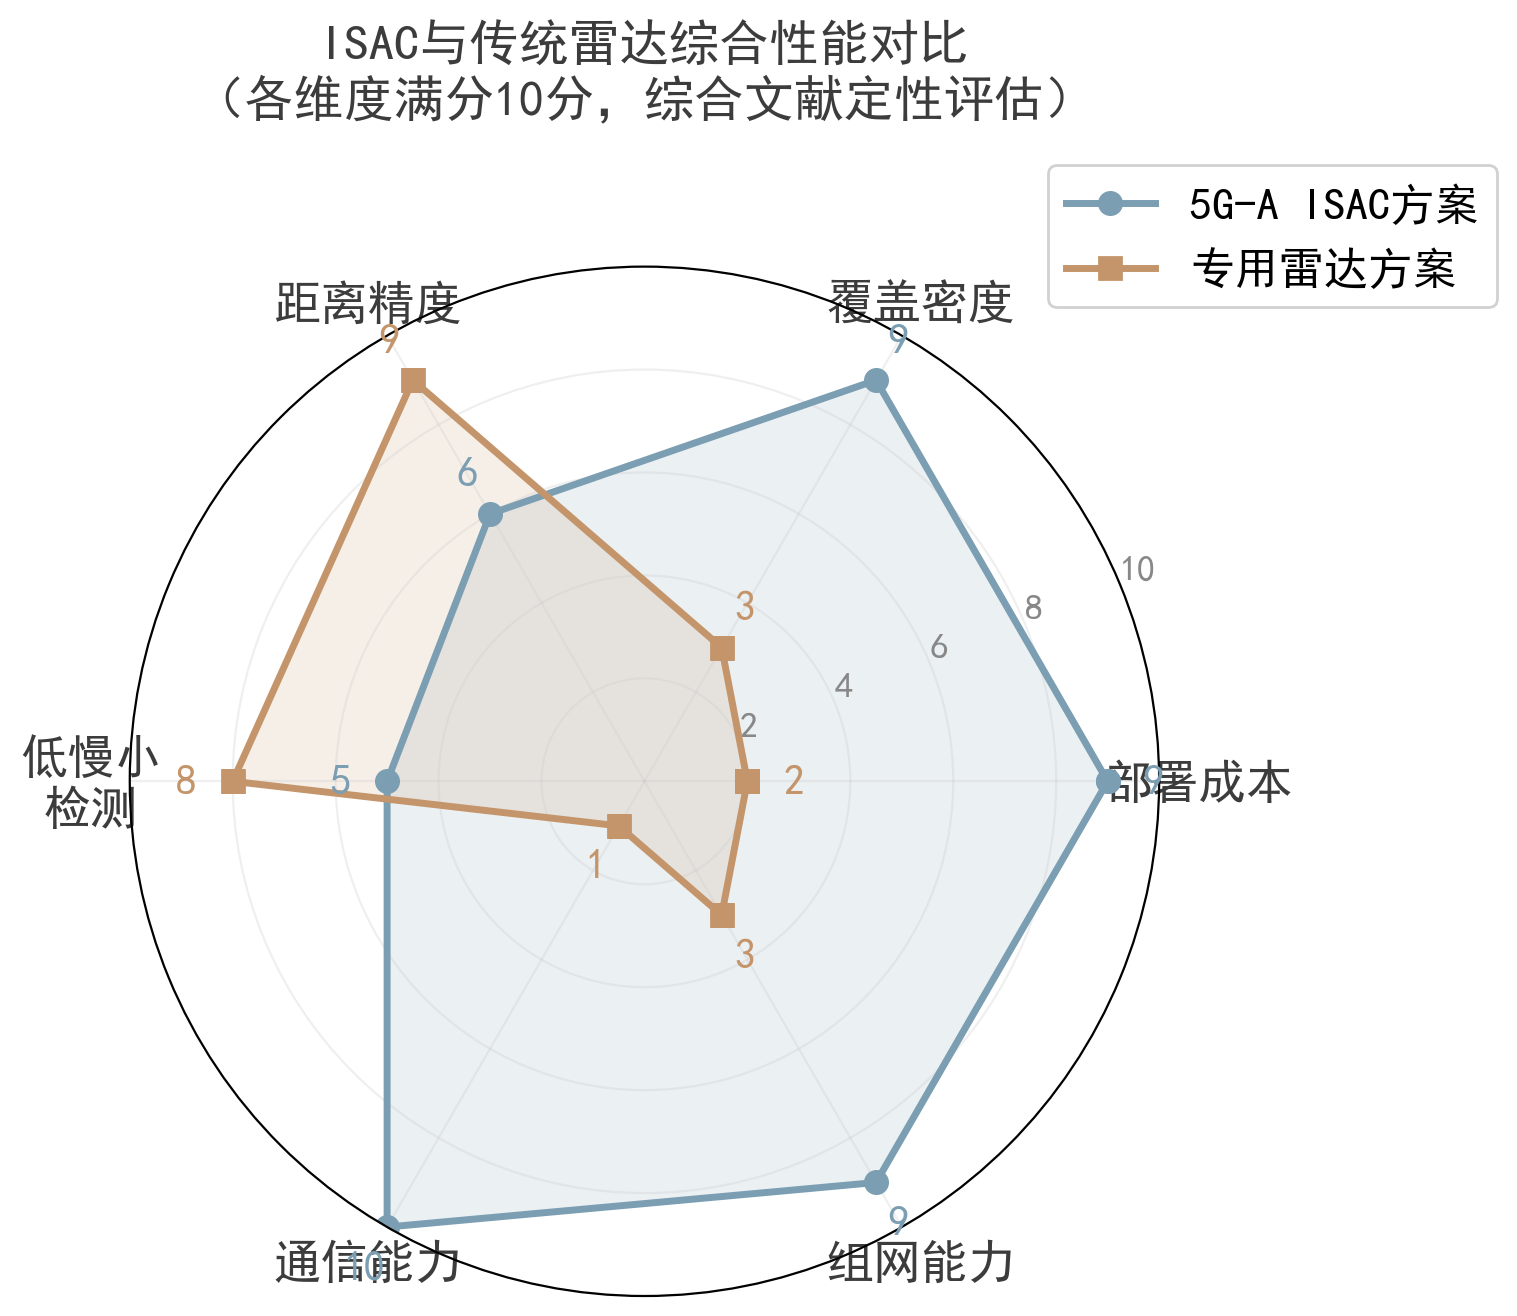
\includegraphics[width=0.6\textwidth]{isac_vs_radar.png}
  \caption{ISAC与传统雷达综合性能雷达图}
  \label{fig:radar}
\end{figure}

ISAC方案在部署成本、覆盖密度、通信能力和组网能力等维度具有显著优势，适合\textbf{广域低空监管}；传统雷达在距离精度和低慢小目标检测方面仍占优，适合\textbf{要地防护}。两者并非替代关系，而是可以形成互补的协同监管体系。

\subsection{不同高度层的感知需求}

\begin{table}[H]
\centering\caption{不同高度层的感知需求分析}\label{tab:altitude}
\begin{tabular}{ccccc}
\toprule
高度层 & 应用场景 & 典型目标 & 定位精度 & 刷新率 \\
\midrule
$<$120\,m & 外卖/快递配送 & 小型多旋翼 & $<$3\,m & 1\,Hz \\
120--300\,m & 物流运输/巡检 & 中型固定翼 & $<$10\,m & 0.5\,Hz \\
300--600\,m & 城际飞行/eVTOL & 载人飞行器 & $<$20\,m & 0.2\,Hz \\
\bottomrule
\end{tabular}
\end{table}

\subsection{本章小结}
国内三大运营商的试点实践表明，ISAC低空方案已从概念验证进入规模化试点部署阶段。ISAC方案在广域覆盖和成本效益方面具有不可替代的优势，与传统雷达形成互补格局。

\section{挑战与展望}

\subsection{现存技术瓶颈}

尽管ISAC技术发展迅速，仍面临以下关键挑战：

\textbf{（1）自干扰消除的工程化难题。}100\,dB以上的宽带自干扰消除在工程实现中面临多重困难：功率放大器（PA）的AM/AM和AM/PM非线性效应导致数字域残余干扰难以精确建模；宽带系统中频率选择性自干扰信道的实时跟踪增加了计算复杂度；温度漂移和器件老化导致射频域对消电路需要频繁校准。

\textbf{（2）通信与感知的性能权衡。}有限的时频资源和发射功率需要在通信QoS与感知探测性能之间寻找帕累托最优。波束赋形中，通信波束需跟踪用户，感知波束需扫描目标区域，联合设计需要解决空间域资源的动态分配问题。

\textbf{（3）非合作目标的检测稳定性。}无人机的RCS随姿态角剧烈变化（可达20\,dB以上起伏），且小型多旋翼的RCS通常低于$-15$\,dBsm，导致在杂波环境中检测概率不稳定，虚警率和漏检率难以同时控制。

\subsection{未来演进方向}

ISAC技术的未来演进呈现三大趋势：

\textbf{（1）AI辅助感知。}利用深度学习替代传统CFAR检测器，如基于卷积神经网络（CNN）的Range-Doppler图目标检测，可在低信噪比条件下提升5--8\,dB的检测增益。同时，基于循环神经网络（RNN/LSTM）的轨迹预测可实现目标行为意图识别，从"检测-定位"的低层感知上升到"识别-理解"的语义感知层面。

\textbf{（2）RIS增强ISAC。}智能超表面（Reconfigurable Intelligent Surface, RIS）通过大量低成本反射单元实现对电磁波传播环境的可编程控制。在ISAC场景中，RIS可以：(a) 创建虚拟视距（Virtual LoS）路径，扩展非视距条件下的感知覆盖；(b) 增强目标回波信号强度，提升弱目标检测能力；(c) 形成空间分集，改善角度估计精度。

\textbf{（3）6G原生感知。}6G系统的目标是在空口设计之初就将感知作为原生能力纳入（Sensing-by-Design），而非5G-A阶段的"通信优先、感知叠加"模式。这意味着新的波形设计（如OTFS用于高多普勒场景）、新的帧结构（感知与通信时隙动态切换）和新的网络架构（感知即服务, Sensing-as-a-Service）。

\subsection{总结}

本报告以低空物联网为应用背景，对5G-A通感一体化技术进行了系统性的研讨分析。从OFDM雷达信号模型与2D-FFT算法的推导与仿真验证，到3GPP R18/R19/R20标准化进展的梳理，再到IoT平台端到端五层架构的设计和MQTT/CoAP/LwM2M协议选型分析，最后对三大运营商的低空试点和ISAC与传统雷达方案进行了对比评估，形成了"物理层感知$\to$数据上报$\to$平台处理$\to$应用驱动"的完整分析闭环。仿真结果表明，5G NR标准参数下的ISAC系统（$N_{\mathrm{CPI}}=14$时隙跨时隙处理）可实现1.5\,m距离分辨率、4.4\,m/s速度分辨率和5\,km探测距离，满足低空无人机监管需求。产业实践证明了ISAC方案的商业可行性。随着AI、RIS等使能技术的成熟和6G标准化的推进，通信感知一体化将成为未来移动通信网络的标配能力。


\begin{thebibliography}{99}

\bibitem{liu2022} Liu F, Cui Y, Masouros C, et al. Integrated sensing and communications: Toward dual-functional wireless networks for 6G and beyond[J]. IEEE Journal on Selected Areas in Communications, 2022, 40(6): 1728-1767.

\bibitem{tr22837} 3GPP TR 22.837. Feasibility study on integrated sensing and communication[S]. V19.2.0, 2024.

\bibitem{tr38857} 3GPP TR 38.857. Study on NR-based sensing[S]. V18.0.0, 2024.

\bibitem{zhang2022} Zhang J A, Rahman M L, Wu K, et al. Enabling joint communication and radar sensing in mobile networks—A survey[J]. IEEE Communications Surveys \& Tutorials, 2022, 24(1): 306-345.

\bibitem{imt2030} IMT-2030 (6G) 推进组. 通信感知一体化技术研究报告[R]. 2023.

\bibitem{cmcc} 中国移动研究院. 5G-A通感一体低空网络技术白皮书[R]. 2024.

\bibitem{sturm2011} Sturm C, Wiesbeck W. Waveform design and signal processing aspects for fusion of wireless communications and radar sensing[J]. Proceedings of the IEEE, 2011, 99(7): 1236-1259.

\bibitem{caict} 中国信通院. 低空经济发展研究报告(2024年)[R]. 2024.

\bibitem{wild2021} Wild T, Braun V, Viswanathan H. Joint design of communication and sensing for beyond 5G and 6G systems[J]. IEEE Access, 2021, 9: 30845-30857.

\bibitem{huawei} 华为技术有限公司. 5G-Advanced通感一体技术白皮书[R]. 2023.

\bibitem{cui2021} Cui Y, Liu F, Jing X, et al. Integrating sensing and communications for ubiquitous IoT: Agile design and implementation[J]. IEEE Internet of Things Journal, 2021, 8(15): 11876-11890.

\bibitem{wymeersch2022} Wymeersch H, Shrestha D, de Lima C M, et al. Integration of communication and sensing in 6G: a joint industrial and academic perspective[C]. IEEE 33rd PIMRC, 2022: 1-7.

\bibitem{zte2024} 中兴通讯. 5G-A通感融合低空解决方案白皮书[R]. 2024.

\bibitem{mqtt} OASIS. MQTT Version 5.0[S]. OASIS Standard, 2019.

\bibitem{coap} Shelby Z, Hartke K, Bormann C. The Constrained Application Protocol (CoAP)[S]. RFC 7252, IETF, 2014.

\bibitem{lwm2m} Open Mobile Alliance. Lightweight M2M Technical Specification v1.2[S]. OMA, 2022.

\end{thebibliography}

\end{document}
